\section{Overview of Our Approach}\label{sec:walg}
\begin{figure*}
\centering
    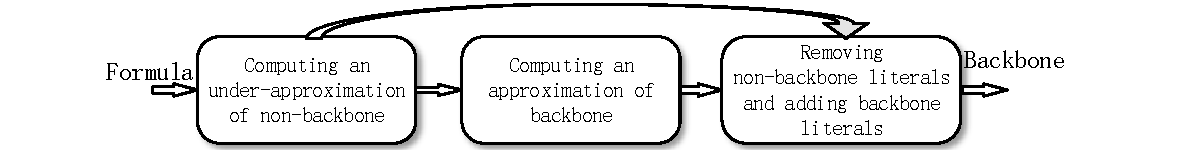
\includegraphics[scale=0.9]{Framework}
   \caption{Overview of our approach}
   \label{flow}
\end{figure*}

In this section, we present the overview of our approach \tool which is depicted in Figure
\ref{flow}. \tool comprises three components. Taking a satisfiable formula
$\Phi$ as an input, \tool first computes an under-approximation $\NBLap(\Phi)\subseteq \NBL(\Phi)$ of the non-backbone of
$\Phi$. Then, \tool computes an approximation $\BLap(\Phi)$ of the backbone of $\Phi$ based on the set $\NBLap(\Phi)$, where each literal in $l\in \BLap(\Phi)$ has a high possibility to be a backbone literal of $\Phi$.
Finally, \tool removes non-backbone literals from $\BLap(\Phi)$ and adds backbone literals into $\BLap(\Phi)$ to compute the exact backbone of $\Phi$.

\medskip
\noindent{\bf Computing an under-approximation of non-backbone.}
Given a satisfiable formula $\Phi$, we first compute a model $\lambda$ of $\Phi$ by calling a SAT solver.
From the model $\lambda$, we can compute a base under-approximation of non-backbone.
Later, we apply a Greedy-based algorithm to add more non-backbone literals into the base under-approximation, which results in the
under-approximation $\NBLap(\Phi)$.



\medskip
\noindent{\bf Computing an approximation of backbone.}
At this step, we apply an improved Whitening-based algorithm to compute the approximation $\BLap(\Phi)$.
The improved Whitening-based algorithm is an extension of the Whitening-based algorithm proposed by \cite{LMZ09} which
was used to compute \emph{frozen variables}, that are the variables whose values are fixed in a non-singleton set of models.
We use the Whitening-based algorithm of \cite{LMZ09} to compute the approximation $\BLap(\Phi)$ in which some non-backbone literals are removed by
a heuristic approach.


\medskip
\noindent{\bf Removing non-backbone literals and adding backbone literals.}
Finally, we first iteratively select one literal $l$ from $\BLap(\Phi)\setminus \NBLap(\Phi)$ such that $\lambda \models \neg l$ and test whether
$l$ is a backbone literal or not by checking the satisfiability of $\Phi\wedge l$. Intuitively, literals in $\BLap(\Phi)\setminus \NBLap(\Phi)$ have a high probability to be backbone literals.
If $\Phi\wedge l$ is satisfiable, then $l$ is a non-backbone literal.
Otherwise, $l$ is a backbone literal. Then, we do the same testing for literals from $\Lit(\Phi)\setminus (\NBLap(\Phi)\cup\BLap(\Phi))$.




\section{Computing $\NBL_u(\Phi)$}


We propose two algorithms for computing $\NBL_u{\Phi}$. The first algorithm computing \MBNB.
Second one \HBNB....

\MBNB computes a complete non-backbone literals set of a given model.
It extracts the relation between literals and clauses, and generate a new model by applying single model rotation.
The satisfiability of an assignment generated by single model rotation is related with the literal that complemented in the rotation. If a complementing a literal won't make any clause unsatisfiable, then a new model is generated. It's obvious that is there are at least two satisfied literal in a clause, then a new assignment generated by complementing one of the literals won't change the satisfiability of this clause. Therefore, by only complementing such literals, new models obtained from single model rotation.

\HBNB computes extends the result of \MBNB with chain model rotation. With multiply rotations, we generate more models with from the initial model. It employs four heuristic depth first searches using Greedy strategies to find virous possible combinations of model rotation. The search is guided by the least/most coverage of literals which indicates the frequency of literals, and the maximal/minimal ratio of literals number to total length of clauses that contain the literal which indicated the importance of the literal to the formula.

\medskip
Based on $\NBL_u{\Phi}$, we apply optimized Whitening Algorithm to compute an approximation of backbone literals by eliminating one of the pattern that cause a false positive of Whitening Algorithm.
We observe that Whitening Algorithm fail to recognize non-backbone literals when there is a large proportion of clauses that only have unique satisfied literal to a given model. We rule out non-backbone literals in this situation by distinguishing a special pattern among them. Among a group of clauses that only contain unique satisfied literal, there may exists a possible model rotation chain. By complementing the unique satisfied literal and more literals in each clause, another satisfied literal may emerge.
....

\medskip

% The basic idea is that if a clause is only satisfied by exactly one literal, no models can be obtained by only complementing the unique satisfied literal. Therefore, if a literal $l$ is not a unique satisfied literal for any clause, a new model $\lambda[l\mapsto\neg\lambda(x)]$ can be obtained. Literal $l$ is a non-backbone literal and will be added to $\NBL_u$.  Besides clauses-literals coverage analysis, we also propose different estimating strategies to extend and find more non-backbones. The strategies is a depth first search approach based on literals weights.
% We leverage whitening algorithm\cite{Par03,LMZ09} to extend the set of $\NBL_u$ to an estimation of backbones literals $\HDBS$ by complementing the result set of whitening algorithm. We refine $\HDBS$ iteratively by exploring model rotation chains. In the end, $\HDBS$ will be an estimation that literals in it are highly likely to be backbones.
%With $\NBL_u$, we are capable to estimate $\HDBS$. $\HDBS$ is initialized with the complement of $\NBL_u$, extensions are achieved by an iterative generation of a clauses estimation, called $\NBC$. For a clause $\phi$ that contains at least one literal $l\in\NBL_u$ or $\neg l \in\NBL_u$,  $\phi$ is added to $\NBC$. Given a model $\lambda$, for a literal $l\models\lambda, l\notin\NBL_u$, if $l$ appears in $\phi\notin\NBC$, $l$ is added to $\HDBS$.



\subsection{An Na\"{\i}ve Algorithm}
Definition.  Lemma.  Intuition. Proof.
\begin{definition}[Free Literals of a Given Model]
Given a formula $\Phi$, a model $\lambda\models\Phi$, a free literal $l\in\Lit(\Phi)$ is a literal such that a new model will generated by complementing $l$, i.e., $\lambda[l\mapsto\neg l]\models\Phi$.
\end{definition}

\begin{lemma}[Free Literals]
Given a formula $\Phi$, a model $\lambda\models\Phi$, a literal $l\in\Lit(\Phi)$ is a \emph{free literal} iff $\forall\phi\in\Phi, l\in\phi\wedge\lambda\models l \Longrightarrow \exists l'\in\phi, l'\neq l\wedge\lambda\models l'$.
\end{lemma}

The satisfiable problem trying to find an assignment that satisfy each clause in a given formula. For a clause that satisfied by the given model, it will change to unsatisfiable or maintain satisfiable when the model changes. We try to make every clause maintains satisfiable and generate a new model by negating the assignment of only one literal.It's trivial that clauses will maintain satisfiable when the complementing literal doesn't appear in the clause. For clauses that contain the changing literal, satisfiable will be maintained iff there is at least another literal which continues assigning the clause to TRUE. Therefore, if a literal only satisfy clauses that have at least two satisfied literals, it's safe to conclude that it's a free literal.

According to the definition of backbone, it's obvious that the set of free literals is a subset of $\NBL(\Phi)$.
\begin{proof}
\label{pro:free literal}
Given a formula $\Phi$, a model $\lambda\models\Phi$. 
Suppose a literal $l\in\Lit(\Phi)$ is a free literal. If $l$ never shows up in any clause (trivial), then there is no such $\phi\in\Phi$ such that $l\in\phi\wedge\lambda\models l$, $\exists l'\in\phi, l'\neq l\wedge\lambda\models l'$ always holds. If $l$ shows up in some clauses, then there is a new model $\lambda[l\mapsto\neg l]\models\Phi$, no clause changes to unsatisfiable because of the changing of $l$. It means that $\forall\phi\in\Phi$, if $l\in\phi$, there must exists another literal $l'\neg l$, assigning $\phi$ to TRUE. Therefore, $\forall\phi\in\Phi, l\in\phi\wedge\lambda\models l \Longrightarrow \exists l'\in\phi, l'\neq l\wedge\lambda\models l'$.

Suppose a literal $l\in\Lit(\Phi)$, if $\forall\phi\in\Phi, l\in\phi\wedge\lambda\models l \Longrightarrow \exists l'\in\phi, l'\neq l\wedge\lambda\models l'$, it means that for every clause that containing $l$, the satisfiable will maintain when changing $l$ to its negation by $l'$. Therefore, there must exist a new model $\lambda[l\mapsto\neg l]\models\Phi$.
\end{proof} 

%Whitening Algorithm can't be applied to backbones extraction directly because it suffers from the over-estimation of non-backbones, i.e, backbones can also be selected to the $\NBL_u(\Phi)$ by the Whitening Algorithm. To fix this defect, only a part of Whitening Algorithm is employed.
%Given a model $\lambda$, there is a possibility that more models can be obtained only by complementing several literals in $\lambda$ without calling a SAT solver. According to the theory of satisfiability, a model $\lambda$ is a truth assignment that satisfies every clause in the formula, i.e., there does not exist a clause $\phi$ that contains no literal in model $\lambda$. With a given model $\lambda$, non-backbones estimation approach is able to compute several similar models that only one literal in complemented. The literals that has been complemented are non-backbones.

%\begin{algorithm}
%\SetKwInOut{Input}{Input}
%\SetKwInOut{Output}{Output}
%\SetAlgoShortEnd
%\SetFillComment
%\Input{$\Phi$: a formula}
%\Output{$\NBLap(\Phi)$: under-approximation of non-backbones}

%$\Psi:=\NBLap(\Phi):=\emptyset$\;
%$(b,\lambda):=\SAT(\Phi$)\;
%\lIf{$b==0$} \Return $\Lit(\Phi)$\;
%$\Psi := \Psi\cup\{\phi\in\Phi \mid \exists l_1, l_2\in \phi, l_1\neq l_2 \wedge\lambda\models l_1\wedge l_2\}$\;
%$\NBLap(\Phi):=\{l\in\Lit(\Phi) \mid  \forall\phi\in\Phi: (\lambda\models l\wedge l\in\phi)\Longrightarrow\phi\in\Psi\}\cup \NBLap(\Phi)$\;
%\Return $\NBLap(\Phi)$\;
%\caption{Non-backbones under-approximation}
%\label{alg:no-loop-w}
%\end{algorithm}

%Given a formula $\Phi$, Algorithm \ref{alg:no-loop-w} computes a set of backbone literals $\NBL_u(\Phi)$ which is a under-approximation of $\NBL(\Phi)$.
%Algorithm \ref{alg:no-loop-w} maintains a set $\Psi$ of clauses and a set of candidate literals of $\NBL_u(\Phi)$, both of them are initialized to $\emptyset$ at Line $1$.
%At Line $2$, an off-the-shelf SAT Solver is called which returns a pair $(b,\lambda)$, where $b$ denotes whether $\Phi$ is satisfiable or not. If $b$ is TRUE, then $\lambda$ is an assignment that satisfies
%$\Phi$. If $b$ is FALSE, $\lambda=\emptyset$, Algorithm \ref{alg:no-loop-w} terminates and returns the set $\Lit(\Phi)$ at Line $3$.
%The Loop at Lines $4-6$ iteratively updates the sets $\NBL_u$ and $\Psi$ for each clause $\phi\in\Phi$. For each clause $\phi\in\Phi$, if there are at least two literals in $\phi$
%that are satisfied by the assignment $\lambda$, then the clause $\phi$ is added into $\Psi$ at Line $5$. If there is a literal that only satisfy clauses in $\Psi$, the literal is added into $\NBL_u(\Phi)$ at Line $6$.

%\begin{lemma}
%Given a satisfied formula $\Phi$, a model $\lambda$. Let $\NBL(\Phi)$ be the non-backbones of $\Phi$.
%$x\in\Lit(\Phi), x\in\NBL(\Phi)$ iff $\exists\lambda'\models\Phi, \lambda\neq\lambda',
%\lambda(x)=\neg\lambda'(x)$.
%\end{lemma}\label{lem:nBL}
%\begin{proof}
%Suppose literal $x\in\Lit(\Phi)\in\NBL(\Phi)$, according to the definition of $\NBL(\Phi)$,
%it must exist two satisfied $\lambda, \lambda'\models\Phi$
%such that $\lambda(x)=\neg\lambda'(x)$, i.e.,
%$\forall x\in\NBL(\Phi)\Longrightarrow\exists \lambda\neq\lambda', \lambda(x)=\neg\lambda'(x), \lambda\models\Phi,\lambda'\models\Phi$.

%Suppose $\lambda, \lambda'$ are two satisfied assignments for a formula $\Phi$,
%$\lambda(x)=\neg\lambda'(x)$.
%According to the definition of $\NBL(\Phi)$, $x$ is in $\NBL(\Phi)$.
%\end{proof}

%\begin{theorem}
%Given a satisfiable formula $\Phi$, let $\NBL_u(\Phi)$ be the set of variables obtained by applying Algorithm \ref{alg:no-loop-w}, then $\NBL_u(\Phi)\subseteq\NBL(\Phi)$.
%\end{theorem}
%\begin{proof}

%Given a satisfied formula $\Phi$, a satisfied assignment $\lambda\models\Phi$.
%Suppose literal $x\in \NBL_u(\Phi)$, let $\Phi_{x}$ be the set of clauses that uses $x$.

%Since $\Phi$ is a satisfied formula, according to the theory of satisfiability, it must exist at least one model $\lambda\models\Phi$. It exists a model $\lambda'=\lambda[x\mapsto\neg\lambda(x)]$, $\lambda'\models\Phi\setminus\Phi_{x}$.
%For every clause $\phi\in\Phi_{x}$, there exists another ${x_1}$, $x\neq x_1$ such that $\lambda(x_1)\models\phi$ (Line $5,6$), $\lambda'(x_1)=\lambda(x_1)$ therefore $\lambda'\models\Phi_{x}$.
%For every clause $\phi\in\Phi_{\neg x}$, $\lambda(x)\not\models\phi$, it exists another ${x_2}$, such that $\lambda(x_2)\models\phi$ (Line $7$), $\lambda'(x_2)=\lambda(x_2)$, therefore $\lambda'\models\Phi_{\neg x}$.
%According to the above proof $\lambda'\models\Phi\setminus\Phi_{x}\cup\Phi_{x}\cup\Phi_{\neg x}=\Phi$.
%According to Lemma \ref{lem:nBL}, $\exists \lambda, \lambda'\models\Phi, \lambda(x)=\neg \lambda'(x)\Longrightarrow x\in\NBL(\Phi)$.
%\end{proof}

%In this section, we proved that there is no backbones in $\NBL_u(\Phi)$, it's safe to directly remove the literals in $\NBL_u(\Phi)$ from backbones estimation.


\subsection{Heuristic-based Algorithm}

%With different models returned by MINISAT, the result of the algorithm in previous section diverged. To shrink the gaps, greedy based literals selection strategies are proposed. With a given literals selection strategy, a chain of literals can be complemented at the same time. In other words, a chain of models will be obtained by the changing assignemnets of literals, coverage of clauses for each literals are updated simultaneously. More models will be generated in this way.

We apply a Greedy-Based Algorithm with different heuristic searching to extend the result of free literals and refereed as $\NBLap$. We leverages Greedy to depth first searches. The quota we choose are frequency represented by the number of appearance of a literal and the entropy represented by the ratio of appearance number of a literal to the total length of clauses that contains the literal. Each quota guided a Greedy search with maximal or minimal value.

\begin{algorithm}
\SetKwInOut{Input}{Input}
\SetKwInOut{Output}{Output}
\SetAlgoShortEnd
\SetFillComment
\Input{$\Phi$: a formula, $\lambda$: a model, free literals of $\lambda$}
\Output{$\NBLap$: under-approximation of non-backbones}
$\NBLap$:=free literals of $\Phi$ to a given model $\lambda$\;
\Repeat {No Update of $\NBLap$}{
    select a list of literals using Greedy heuristic\;
    change the selected literal one by one to generate a new model\;
    add new free literals to $\NBLap$.
    % $\Psi=\Psi\setminus\{\phi\in\Psi,\lambda(x)\models\phi, |\{l\in\phi \mid \l\models\phi\}|=2\}$\;
    % $\Psi=\Psi\cup\{\forall\phi\in\Phi, \neg\lambda(x)\models\phi\}$\;
    % $\lambda=\lambda[x\mapsto\neg\lambda(x)]$\;
    % $\NBL_i(\Phi)=\NBL_i(\Phi)\cup\{x\in\Lit(\Phi) \mid \forall\phi\in\Phi: \lambda(x)\models\phi\Longrightarrow\phi\in\Psi\}$\;
}
\Return $\NBLap$\;
\caption{Heuristic extension for computing $\NBL_u$}\label{alg:whiten-greedy}
\label{alg:wal}
\end{algorithm}
% Heuristic searching strategies that used at Line $9$ in Algorithm \ref{alg:whiten-greedy} are:
% \begin{enumerate}
    %\item Let $|\Lit(\phi)|$ be the number of clauses that used in a clause $\phi\in\Phi$, for every literal $x\in \NBL_1(\Phi)$, select exactly one literal at each iteration of the loop such that $\max\{|\phi_{x}|\}$.
    %\item Let $|\Lit(\phi)|$ be the number of clauses that used in a clause $\phi\in\Phi$, for every literal $x\in \NBL_2(\Phi)$, select exactly one literal at each iteration of the loop such that $\min\{|\phi_{x}|\}$.
    %\item Let $|\Lit(\phi)|$ be the number of clauses that used in a clause $\phi\in\Phi$, let $|\Phi_{x}|$ be the total length of clauses $\phi\in\Phi$ that used $x$, i.e., $|\Phi_{x}|=\sum\{\phi\in\Phi \mid \phi\in\Phi_{x}\}$ for every literal $x\in \NBL_3(\Phi)$, select exactly one literal at each iteration of the loop such that $\max\{|\phi_{x}|\div|\Phi_{x}|\}$.
    %\item Let $|\Lit(\phi)|$ be the number of clauses that used in a clause $\phi\in\Phi$, let $|\Phi_{x}|$ be the total length of clauses $\phi\in\Phi$ that used $x$, i.e., $|\Phi_{x}|=\sum\{\phi\in\Phi \mid \phi\in\Phi_{x}\}$ for every literal $x\in \NBL_4(\Phi)$, select exactly one literal at each iteration of the loop such that $\min\{|\phi_{x}|\div|\Phi_{x}|\}$.
% \end{enumerate}

The algorithm take the free literals of a given model as input and assigned to $\NBLap$ as shown in Line 1. From Line 2 to Line 6, $\NBLap$ is expanded. Different heuristic are chosen at Line 3 to select a list of literals and changing the assignment of them with a increased or decreased order. 

In order to generate virous models from a given model, we need to negate more literals. We generate consecutive models by changing the assignments of literals one by one. Since enumerating every model of a satisfied formula is known as a NP hard problem, many heuristic strategies are applied to model generation. The selection of literals paly a vital role in it, with a different changing decisions, different models are generated. We take the idea of term frequency from statistic research, namely Term Frequency-Inverse Document Frequency(TF-IDF). In our context, literals are regarded as terms, clauses are regarded as documents. The frequency of terms are represented as the appearance number of literals. The inverse document frequency of a literal is represented as the ratio of appearance number to the total length of clauses that contained the literal.

\begin{lemma}
The result of Algorithm \ref{alg:wal} is a subset of $\NBL$.
\end{lemma}
\begin{proof}
For every model generated during the algorithms, the free literals is added to the result set of Algorithm \ref{alg:wal}.
Since free literals is a subset of $\NBL$, the result is also a subset of $\NBL$.
\end{proof}
% The final $\NBL_u(\Phi)$ result of our approach is $\NBL_u=\bigcup_{i=1}^4 \NBL_i(\Phi)\cup \NBL$.

% Compared with $\NBL_u(\Phi)$, the strategies applied in this sections can be viewed as four different kinds of depth-first search, while $\NBL_u(\Phi)$ is a width-first search. With different search methods, we are able to explore more paths and obtain more diverse models.

\section{Computing $\HBL(\Phi)$}



\begin{algorithm}
\SetKwInOut{Input}{Input}
\SetKwInOut{Output}{Output}
\SetAlgoShortEnd
\SetFillComment
\Input{$\Phi$: a formula}
\Output{$\HDBS(\Phi)$:Backbones Estimation of $\Phi$}


$\NBC=\HDBS(\Phi)=\emptyset$\;
$\NBL_e=\NBL_u$\;
$(b,\lambda)=\SAT(\Phi$)\;
\lIf{$b==0$} \Return $\Lit(\Phi)$\;
\For{$\phi\in\Phi$}{
    $\NBC = \NBC\cup\{\phi\in\Phi \mid \exists x\in\phi, x\in\NBL_u\}$\;
    $\NBL_e(\Phi)=\NBL_e(\Phi)\cup \{x\in\Lit(\Phi) \mid \forall\phi\in\Phi: \lambda(x)\models\phi\Longrightarrow\phi\in\NBC\}$\;
}
\Repeat{No Update of $\NBL_e$}{
    $\NBC = \NBC \cup \{\phi\in\Phi\setminus\NBC \mid \exists x\in\NBL_e(\Phi)\vee\exists\neg x\in\NBL_e, x\in\Lit(\phi)\}$\;
    $\NBL_e(\Phi) = \NBL_e(\Phi) \cup \{x\in \Lit(\Phi) \mid \forall\phi\in\Phi: \lambda(x)\models\phi\Longrightarrow\phi\in\Psi\}$\;
}
$\HDBS=\Lit(\Phi)\setminus\NBL_e(\Phi)$\;
\For{$x\in\HDBS(\Phi)$}{
    $k=1$\;
    $\Phi_{x}^0=\{x\}$\;
    \Repeat {$\Phi_{l_x}^k=\Phi$}{
        $\Phi_{x}^k=\{\phi\in\Phi \mid \neg\Lit(\Phi_{x}^{k-1})\in\phi\}$\;
        \If{$\neg x\in\Lit(\Phi_{x}^k)$}{
                $\HDBS(\Phi)=\HDBS(\Phi)\setminus\{x\}$\;
                $Break$\;
        }
        $k=k+1$\;
    }
}
\Return $\HDBS(\Phi)$\;
\caption{Backbones Estimation of $\Phi$, $\HDBS(\Phi)$}
\label{alg:nBLo}
\end{algorithm}

To increase the density of backbones, we propose $\HDBS$ approach to estimate literals that are highly likely to be backbones. In other words, $\HDBS$ increase the backbones density by estimations. There are two parts of $\HDBS$ approach. The first part extends $\NBL_u$ to find more likely backbone literals. The new estimation of variables is called $\NBL_e$. It relax the constraint of estimation selection constraints.

The second part of $\HDBS$ approach is a deletion based approach. $\HDBS$ is initialized with the complement of $\NBL_e$. There is a possibility that there are still non-backbones not in $\NBL_e$. If that happens, there must exist another non-backbone literal that $\NBL_e$ failed to recognise. Then, both of the two literals are added to $\HDBS$, in this way, $\HDBS$ is updated.

Line $5-10$ compute $\NBL_e$. The loop from Line $8-11$ iterative updated $\NBC$ and $\HDBS$.
In Line 9, if a clause $\phi\in\Phi$ contains a literal or its negation $l$ such that $l\in\NBL_u\vee\neg l\in\NBL_u$, $\phi$ is added to $\NBC$.
Given a model $\lambda$, suppose $l\in\phi$, $l\in\lambda$, according to Lemma \ref{lem:nBL}, there exists a model $\lambda'\neq\lambda\models\Phi$. Therefore, clause $\phi$ will be satisfied under any truth assignment of $l$.
Given a model $\lambda$, suppose $l\in\phi$, $\neg l\in\lambda$, according to Lemma \ref{lem:nBL}, there exists a model $\lambda'$ with $\lambda'(l)=\neg\lambda(l)$. It means that clause $\phi$ will be satisfied by $l$ when complementing $\neg l$. Therefore, clause $\phi$ will be satisfied under any truth assignment of $l$. With the updated $\NBC$, $\NBL_e$ is updated in Line 10.

Line 12 initialize $\HDBS$ as the complement of $\NBL_e$, since our goal is to find a group of literals with dense backbones, we want to find non-backbone literals in $\HDBS$ without applying MINISAT. Line 13-22 explains how non-backbones are found in $\HDBS$. Given a literal $l\in\HDBS$, with the pre-condition that $l\not\in\NBL_e$, there doesn't exist tow different model $\lambda$, $\lambda'$, such that $\lambda(l)=\neg\lambda'(l)$. In other words, there must exist another non-backbone literal $x_1\in\HDBS$ in $\Phi_x$, such that $x_1$ complemented together with $x$.
Suppose $\phi_1$, $\phi_2$, $\phi_3$ $\notin\NBC$, suppose $x_1$, $\neg x_1$, $x_2$, $\neg x_2$, $x_3$, $\neg x_3$ $\in\HDBS$, $x_1\in\phi_1, \neg x_2\in\phi_1$, $x_2\in\phi_2, \neg x_3\in\phi_2$, $x_3\in\phi_3, \neg x_1\in\phi_3$.
Given a model $\lambda$, where $\lambda(x_1)=1, \lambda(x_2)=1, \lambda(x_3)=1$. $x_1, x_2, x_3$ are the only satisfied literal in $\phi_1, \phi_2, \phi_3$ respectively.
It can be observed that if $x_1$ is a non-backbone literal, in order to generate a $\lambda'$ that satisfy $\phi_1, \phi_2$ and $\phi_3$, $x_1, x_2, x_3$ have to complemented simultaneously. Based on the observation, line 13-22 tries to find a group of literals that have to complement at the same time to generate a new model.
$\Phi_x^0$ is initialized with the a literal $x\in\HDBS$, and line 17-21 will find the group of literals that have to negate together if $x$ is a non-backbone literal. If there is no literal found by the end of line 22, $x$ will remained in $\HDBS$. In a iterative searching process, $\Phi_x^k$ is computed with the information of k-1 step at Line 17. For each step of $\Phi_x^k$, it stands for the clauses that contains at least one literal that showed up in $\Phi^{k-1}_x$. If the negation literal of $x$ is founded during the search, the search terminates for $x$ and move to next literal in $\HDBS$.

With the above steps, the percentage of backbone literals in $\HDBS$ will be relatively high. With dense backbones $\HDBS$, MEB will achieve the best performance.
\begin{theorem}
The complexity of Algorithm \ref{alg:nBLo} from Line 5 to 23 is in polynomial time.
\end{theorem}
\begin{proof}
Suppose $|\Lit(\Phi)|=m$, $|\cls(\Phi)|=n$.
Suppose the average length of $\phi\in\Phi$ is k, i.e., $|\phi\in\Phi|=k$.
Suppose the average number of clauses that each literals appears is l, i.e., $|\Phi_l|=l$.
For Line 5 to 8, there is a loop for each clause in $\phi\in\Phi$ to test if $\phi$ is in $\NBC$ or not.  The complexity of each iteration is $O(k)$. The complexity of Line 5 to 8 is $O(m*k)$.
For Line 9 to 11, there is a loop for each literal that have been selected to $\NBL_e$. In each iteration of the loop, $\NBC$ is updated with the complexity of $O(1)$. The complexity of Line 10 in the loop is $O(l)$. The worst case is that every literal $l\in\Lit(\Phi)$ have been selected to $\NBL_e$ one by one. The complexity of Line 9 to 11 is $O(m*l)$.
For Line 13 to 23, the complexity of Line 14, 15 is $O(1)$. There is a loop of literals that in $\HDBS$. For the worst case, Line 23 won't be executed until every literal of $\HDBS$ had been visited. In the first iteration of the loop, the complexity of Line 17 is $O(k*l)$. In the second iteration, the complexity of Line 17 is $O(k*l*l)$. In the $i^{th}$ iteration of the loop, the complexity of Line 17 is $O(k*l^i)$. Therefore, the complexity of Line 17 is $O(k*l^n)$. The complexity of Line 18-22 is $O(1)$. The complexity of Line 13 to 23 is $O(l*l^i)$.
As discussed above, the complexity of Line 5 to Line 23 in Algorithm \ref{alg:nBLo} is $O(k*l^i+m*k+m*l)$.
\end{proof}

\medskip
With $\NBL_u$ and $\HDBS$ above, both backbones estimation $\HDBS$ and non-backbones estimation $\NBL_u$ can be obtained.  First of all, $\HDBS$ are tested iteratively by adding one assumption to the formula at a time. In each iteration, MINISAT returns true if the literals in assumptions is a non-backbone or false if the literal is a backbone. The first several MINISAT calls may be slow depending on the complexity of the formula. With more backbones being recognise by the testing, the testing procedure will be dramatically accelerated. After teasing of $\HDBS$, the complement of $(\HDBS\cup\NBL_u)$ is iterative tested one by one, which can be finished in a blink. The flow path of MEB approach is showed in Fig \ref{fig:flow}.


It first start with computing $\NBL_u$ and $\HDBS$. Iterative SAT solver calls are applied to each literal in $\HDBS$, in the flow path, a literal $l$ is marked as tested after the MINISAT call. If MINISAT returns true, then $l$ is marked as backbones. Otherwise, $l$ is a non-backbone and can't contribute to MEB anymore. The complement of $\HDBS\cup\NBL_u$ is the next test candidate set. If every literal of formula is already marked tested, MEB terminates.



\begin{algorithm}
\SetKwInOut{Input}{Input}
\SetKwInOut{Output}{Output}
\SetAlgoShortEnd
\SetFillComment
\Input{$\Phi$: a formula}
\Output{$\BL(\Phi)$:Backbones of $\Phi$}

$\BL=\emptyset$\;
$\Phi'=\Phi$\;
$(b,\lambda)=\SAT(\Phi$)\;
\lIf{$b==0$} \Return $\Lit(\Phi)$\;
\For{$TRUE$}{
    \For{$l\in\lambda$}{
        $\Phi'=\Phi'\wedge\neg l$\;
    }
    $(b, \omega)=\MUC(\Phi')$\;
    \lIf {$b==1$} \Return $\BL(\Phi)$\;
    \If {$b==0$}{
        $\BL=\BL\cup\{l \mid l\in\omega\}$\;
        $\Phi'=\Phi'\setminus\omega$\;
    }
}
\Return $\BL(\Phi)$\;
\caption{Backbones Extracting Using MUC}
\label{alg:MUC}
\end{algorithm}





